\subsection{Projects}
The point is to have two applications that are similar. This way we can see if the SDS brings improvements for the user. For this reason, it is important that both systems are visually indistinguishable from each other. Both systems consist of three views and an optional view that is used to explain the test case task to the user. Therefore, this view is omitted from the count. \\

\begin{figure}[hbtp]
    \centerline{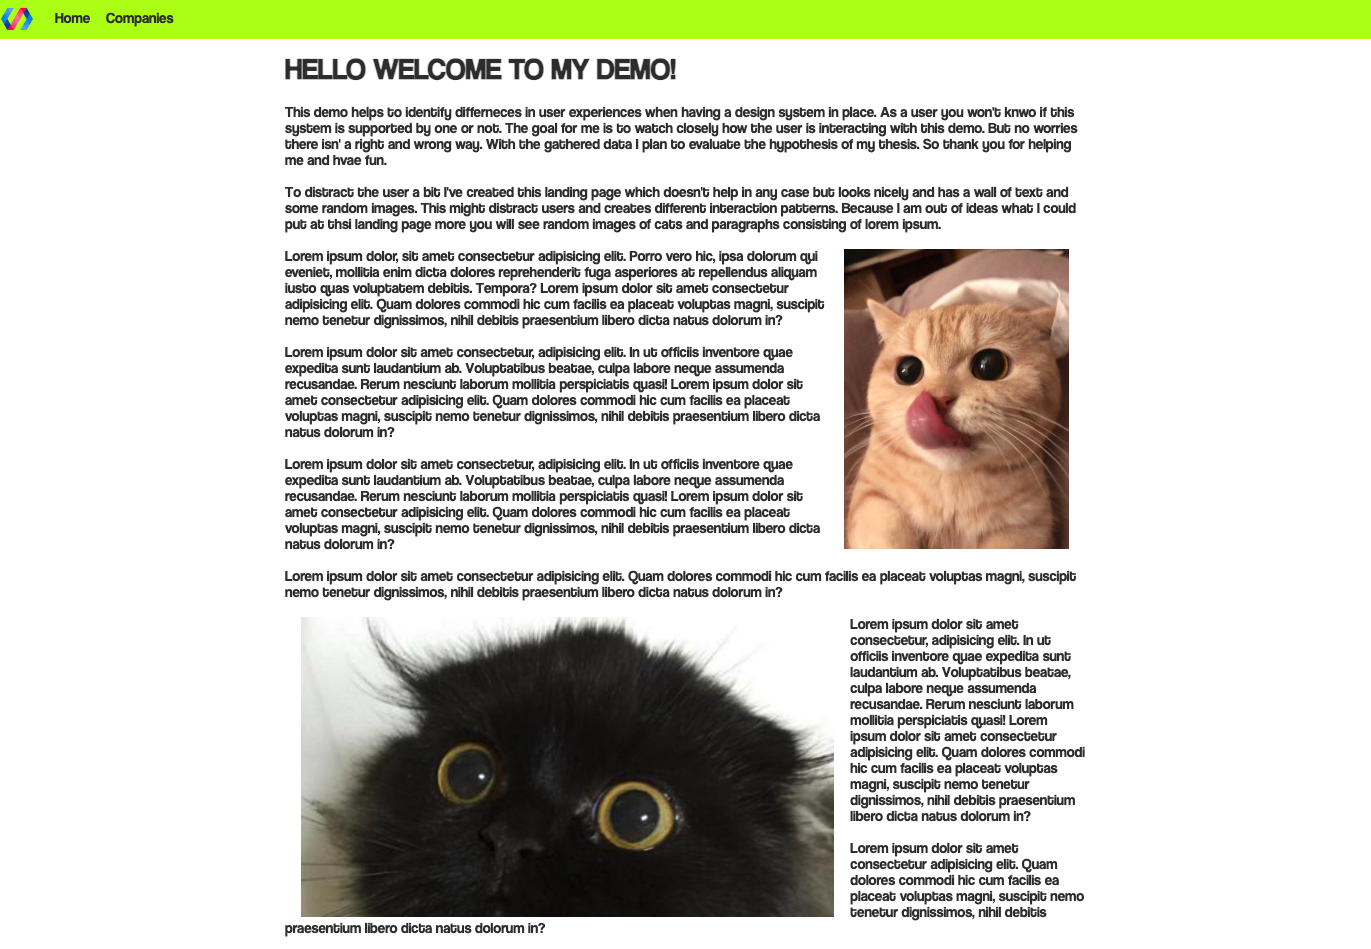
\includegraphics[height=7cm, draft=false]{images/demo_view_landing_page.png}}
    \caption{Landing page of test applications}
    \label{landing_page}
    \end{figure}
The first view (Figure \ref{landing_page}) is the landing page when the user starts the test run. Here the user will find a navigation bar, which is also included in the other two views, to navigate through the application. The main goal of this view is to distract the user. Long paragraphs with sample texts and cat photos are meant to draw the user away. After all, he is supposed to navigate to the second view, the data table, via the upper navigation bar. When the user clicks on "Company", he is redirected to the second view. 
\\

In the second view (Figure \ref{data_table}), the user sees a data table with entries from various made-up companies. Besides the company name, the user finds the current status of the company and a description in the table. The description is also a Lorem ipsum without any relevance. At the top right of the data table, the user finds a button labelled "Add +". This button leads him to the third view. 
\begin{figure}[htbp]
    \centerline{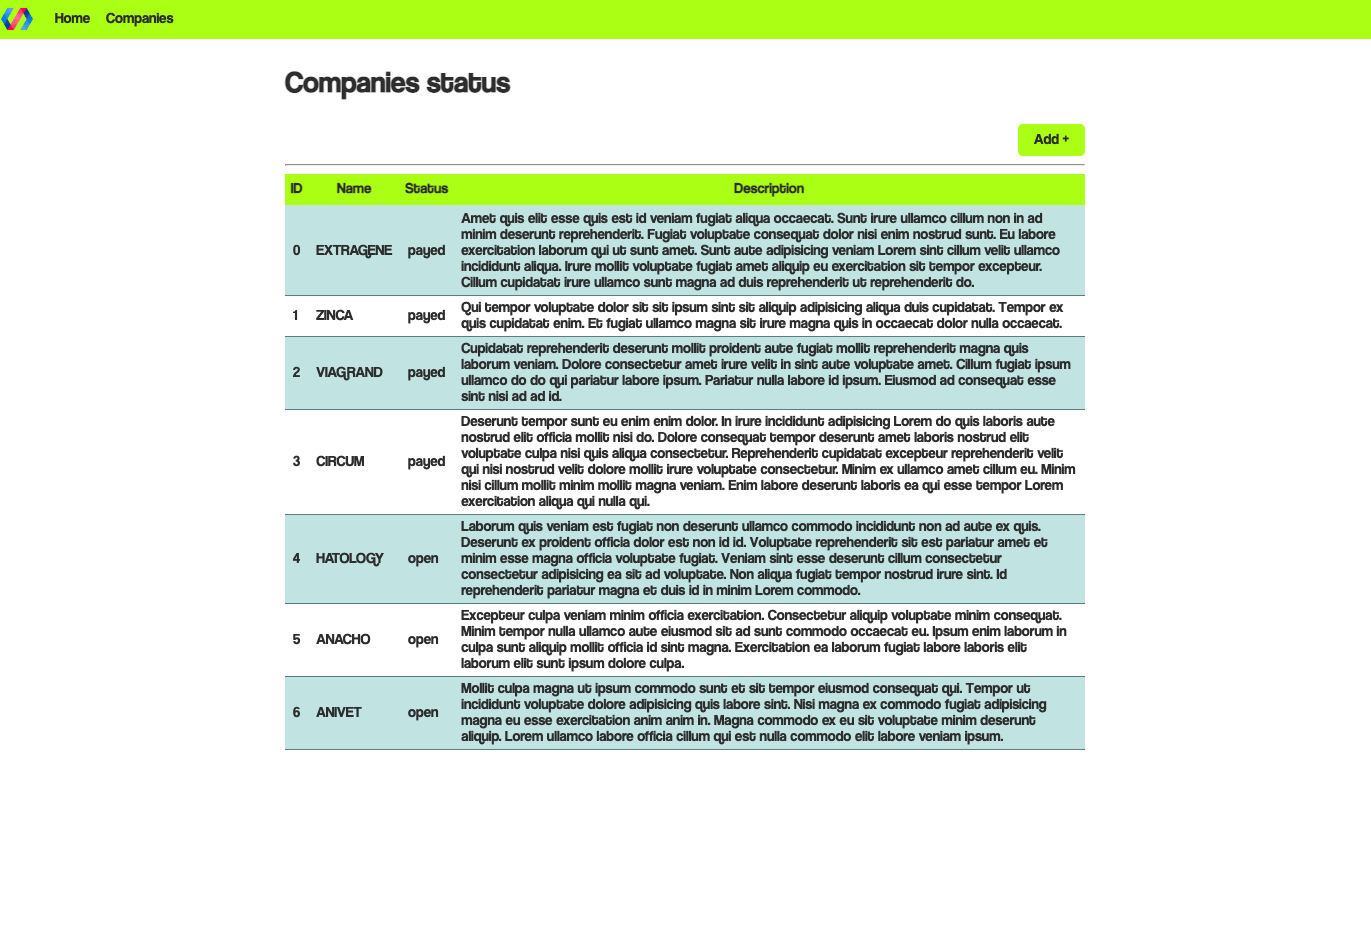
\includegraphics[height=7cm, draft=false]{images/demo_view_data_table.png}}
    \caption{Data table page of test applications}
    \label{data_table}
    \end{figure}
    \\

The last view (Figure \ref{adding_form}) of the sample applications shows a form for adding new data to the table. The form has three inputs for each value corresponding to the table from the second view. All inputs are plain text inputs with no restriction or validation of the inputs. In a real scenario, there would be validation, but due to the limited time frame of this elaboration, this feature is omitted. At the bottom of the form, the user sees a button to save the form. This button is disabled until all input fields are filled with a value. 
\begin{figure}[htbp]
    \centerline{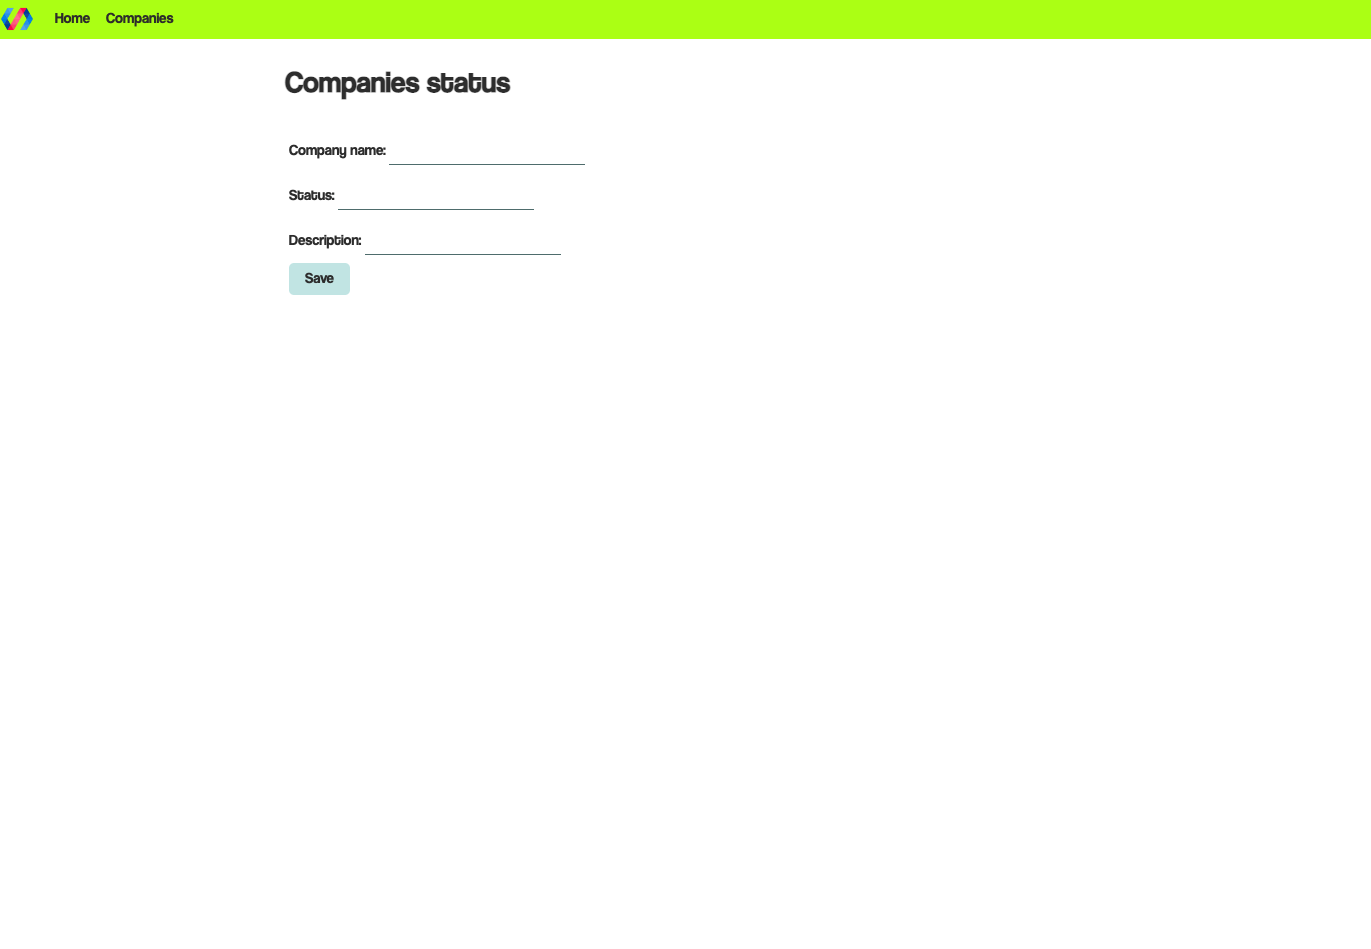
\includegraphics[height=7cm, draft=false]{images/demo_view_form.png}}
    \caption{Data adding view of test applications}
    \label{adding_form}
    \end{figure}
\\

Both applications not only have the same views, but also the same technology stack. They are based on Svelte, a library for building web applications with a small package size. According to the starter guide, we use Rollup as a bundling and compilation tool. So both applications do not differ in terms of technology and build steps. \cite{svelte_svelte_nodate} \\
The only difference between the two systems are the implementation details. The next chapters will therefore explain the structure of each application and how views are created with and without SDS.
\subsubsection{Application using \ac{SDS}}
First, a summary of how to use the \acl{SDS}. To use the web components, the application must import the code that adds the components. In this case, the system contains the bundle described in \ref{SDS_build_and_integration}. This is done via the \texttt{main.ts} file, which is defined as an input file in the rollup configuration. \\
\lstinputlisting[linerange={1-9},firstnumber=1,caption={Bootstrapping of Svelte application with \ac{SDS}},label=BootstrappingAppSDS]{../Code/sds-demo-app/src/main.ts}
As can be seen in Listing \ref{BootstrappingAppSDS}, the bootstrapping of the Svelte application is performed here by creating the Svelte App component and appending it to the body. Also, in line 2, the SDS bundle is imported. This adds the design system components to the application. Now it is possible to use all the web components within the app via the HTML tags defined by \ac{SDS}. \\

After successfully bootstrapping the app, the next step is to look at the Svelte components themselves and how they build the given views. Since the app component is only needed for bootstrapping and initialising the router, another check can be omitted. According to the routing details, the next component to be loaded is Main.svelte. \\
The Main component is responsible for displaying the navigation bar, which can be seen at the top of each displayed view. In addition, it contains a content placholder where other components are displayed. The code of the component shows that web components from the \ac{SDS} are used. Line 7-11 in Listing \ref{MainSvelteSDS} use the navigation bar (\texttt{<saas-navbar>}) and the corresponding navigation bar items (\texttt{<saas-navbar-item>}).
\lstinputlisting[linerange={1-14},firstnumber=1,caption={Main.svelte with \ac{SDS}},label=MainSvelteSDS]{../Code/sds-demo-app/src/components/Main.svelte}
The component takes advantage of the functionality of slots by inserting elements into the navbar component. The web component then takes care of the corresponding display at the top. The Navbar elements inside ensure that the declared navigation links are displayed with the correct styles defined by the design system. A special feature in line 8, Listing \ref{MainSvelteSDS} is the \texttt{<img>} element. This HTML element is responsible for displaying the logo in the upper left corner. The element has a special property called "slot". Its value is set to "logo". The web component of the navigation bar recognizes this slot definition and inserts the image with the expected styles in the navigation bar. \\
Below the code for the navigation bar, lines 12-14, Listing \ref{MainSvelteSDS} contain the code for displaying the content of the application. In addition to the navigation bar web component, the content web component is also provided with the design system. It uses the same logic as the navigation bar by providing a placeholder for elements within that component and applying styles to the content container within the web component. Adjustable by design token within the SDS. The \texttt{<Router>} tag within the content is an imported Svelte component that handles the display of the content according to the visited route. \\
% Home component
% Data component
% Form

\subsubsection{Project without SDS}
